\section{Augmented Foster-Lyapunov Bounds}\label{ch:lyapunov}
The use of Foster-Lyapunov approaches, is often two-fold: They are used to prove ergodicity and to provide sets with a lower bound $1-\epsilon$ on their stationary probability mass.
Often practical methods focus on proving \emph{global} properties of their associated drift \parencite{gupta2014scalable,spieler2014numerical}.
In many models, simple affine functions \parencite{gupta2017finite} and even the identity \parencite{spieler2014numerical} is sufficient.
While such simple forms provide some of the necessary ease of a global analysis, the task of optimizing them with performance in mind, is much more difficult \parencite{milias2014optimization}.\marginpar{\emph{Performance} in this context means least states to cover most stationary probability mass.}

Ideally one would have the best of both worlds: The ease of working with simple forms for the global guarantees of the Foster-Lyapunov criteria and the freedom of choice to fit efficient functions and get sets that are as small as possible.
The approach presented here achieves this by \emph{locally} altering a proposal Foster-Lyapunov function.
The presence of such a valid proposal function is necessarcy for this method.
Such a function can be identified by convex analysis, for example \parencite{gupta2014scalable} or using the approach described by \textcite{spieler2014numerical}.
Using a set of probability $>1-\epsilon$ is identified using such a functional.
On this set, the original function is then replaced by any other lower bounded function.
At the set boundary this supplementary function is \emph{phased out} and we switch back to the original function using some smooth step function.
The choice of such a supplementary function offers much room for experimentation since all the necessary global criteria.
For this function we can, for example, use any polynomial or even more variable models such as neural networks.

The procedure to identify an efficient function is thereby reduced to a simple machine learning problem.
The objective exponentially rewards negative drift yielding tight sets.
Its computation needs, in principle, all points in a sufficiently large set.
For optimization however, we switch to an approach of sampling uniformly from the augmentation set.

This method yields sets that are smaller on the order of $10^3$ for a fixed probability bound over a simple linear functional.
We study neural networks and polynomial templates as candidates for local augmentation.

\subsection{The Drift and its Properties}
The drift \eqref{eq:drift} plays a central role in this chapter.\marginpar{We explain the interpretation and give some basic use of the drift in \autoref{sec:statagg:lyapunov} on page~\pageref{sec:statagg:lyapunov}.}
\begin{equation}
	d(x; g) = Qg(x) = \sum_{j=1}^{n_R} \alpha_j(x) (g(x+v_j) -  g(x))
\end{equation}
An interesting fact about the drift is, that it is invariant to linear transforms to $g$.
That is, for a constant $b\in\mathbb{R}$, we can define $h(x)=g(x)+b$ and \( Qh(x) =Qg(x)\).
Clearly, a positive linear factor $m$ to $g$ factors out, i.e.\ $Q(f\circ g)(x)=mQg(x)$ for $f(x) = mx$, $m>0$.
Consequently, if the drift is scaled by its maximum value, the scaled version is invariant to linear
transforms of $g$:
\begin{equation}
	\frac{Q(f\circ g)(x)}{\max_{x\in\mathcal{S}}Q(f \circ g)(x)}
	=
	\frac{Qg(x)}{\max_{x\in\mathcal{S}}Qg(x)}
\end{equation}
Since the probability bounded sets $C_{\epsilon_{\ell}}$ depend on the scaled drift.
Therefore invariance under linear transformation implies that we cannot change --~especially improve~-- the tightness of the sets by such a transform.

\subsection{Local Substitution}
We use a proved Foster-Lyapunov function as a starting point.
For many relevant reaction networks, simple choices such as L1 or L2 norms are sufficient choices \parencite{spieler2014numerical}.
The resulting sets, however, are typically very large.
Tasks such as computing approximate stationary distributions on truncations set up according to these sets can be very costly.
This cost is exacerbated when a system has to be solved for a lot of different reentry matrices, which is necessary when state-wise bounds on the probability conditioned on a truncation are desired~\parencite{dayar2011bounding}.

We propose to augment the proposal function by a function, that is limited to local influence guided by the initial set.
This supplementary function is phased out asymptotically using a simple sigmoid threshold function
\begin{equation}\label{eq:threshold}
  \gamma_{k,z}(x) = \frac{1}{1+k\exp(-x - z)}\,.
\end{equation}
Thus, in a one-dimensional model the augmented Lyapunov $g'$ function becomes
\begin{equation}\label{eq:thres_lyapunov}
    g'(x) = \gamma_{k,z}(x) g(x) + (1 - \gamma_{k,z}(x)) g^*(x)\,.
\end{equation}
The threshold function $\gamma$ guarantees that $g^*$ vanishes asymptotically.
The drifts $d'$ and $d^*$ are defined accordingly.

\subsection{Illustrating Example}
Consider the example of Model~\ref{model:bd}.
The question is: What makes the perfect Foster-Lyapunov function?
Here, we are interested in the smalled set of states containing the largest amount of stationary probability mass.
\marginpar{The beauty standard may vary for other applications.}
Since we know the stationary distribution to be Poissonian, its standard confidence intervals can be used as a reference.
The confidence interval for level $1-\alpha$ of a Poisson with rate $\mu$ is
\[
\frac{1}{2}P^{-1}(\alpha/2; 2k)\le\mu\leq\frac{1}{2}P^{-1}(1-\alpha/2;{2k+2})\,.
\]
where $P^{-1}(\,\cdot\,; l)$ is the inverse \ac{CDF} of a $\chi^2_{l}$ distribution.
Thus, its the inverse of the regularized gamma function
\[
	\frac{1}{\Gamma(k/2)}\int_0^{x/2} t^{k/2 - 1} e^{-t}\,dt
\]
w.r.t.\ $x$.
This gives us the ``ideal'' intervals $[l_{\epsilon},h_{\epsilon}]$, $(l_{\epsilon},h_{\epsilon})\in\mathbb{N}^2$ such that $\pi_{\infty}([l_{\epsilon},h_{\epsilon}])=1-\epsilon$.
These sets are given as the dark area in \autoref{fig:lya_sets}.
Therefore, the perfect Lyapunov function would coincide with those sets. That is,
a function $g$ such that
\[
%	\left\{x\in\mathcal{S}\mid \frac{\epsilon}{c}Qg(x)> \epsilon - 1\right\}
	C_{\epsilon}
	=
	\left[l_{\epsilon}, h_{\epsilon}\right], \quad \forall\epsilon> 0\,.
\]

Using a simple L2 norm as an initially, i.e.\ $g(x) = x^2$, we obtain a fairly large set.
In Figure~\ref{fig:bd:truncation}, we contrast this result to the solution given by the choice of $g^*(x)=(x - 250)^2$, which gives a much tighter subset with the same guarantees.
In this case, the guarantee is that the sets contain at least 0.9 stationary probability mass.
We further demonstrate how the incorporation $g^*$ into $g$ significantly tightens the set proposed initially.
\begin{figure}[htb]
    \centering
    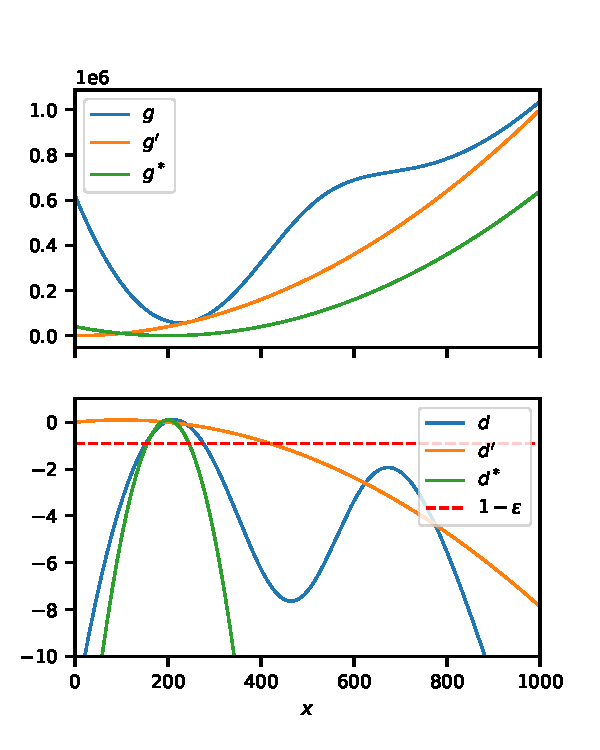
\includegraphics[width=.6\textwidth]{gfx/lyapunov_bd.pdf}
    \caption[Augmented Foster-Lyapunov function]{\label{fig:bd:truncation}Different example Lyapunov functions for Model~\ref{model:bd}. The drifts $d$, $d^*$, and $d'$ are scaled and the appropriate threshold for $\epsilon=0.1$ is given.}
\end{figure}


The benefit of the threshold-based construction \eqref{eq:thres_lyapunov} is that we only require $g^*$ to be non-negative.
All other properties are inherited from the proposal function.
This freedom enables the use of flexible machine learning models to search an efficient $g^*$.


\paragraph{Neural Augmentation}
The characteristics of the augmentation function $g^*$ are typically not known beforehand.
The formulation of augmented Foster-Lyapunov functions only places basic constraints on the function used:
The function needs to be non-negative and an upper bound of the drift has to be known.
Neural networks lend themselves naturally as an extremely flexible functional family.

The central piece of fitting $g^*$ is an objective function.
Since the actual sets, bounded in probability, are defined in terms of their drift, this objective needs to be a function of this drift.
A desirable augmented drift has tight level sets with more emphasis placed on its peak regions.
A natural way to express this prioritization is the objective
\[\sum_{x\in\mathcal{S}}\int_{-\infty}^{d^*(x)}\exp(y)\,dy = \sum_{x\in\mathcal{S}} \exp(d'(x)) \]
based on the scaled augmented drift.

In \autoref{fig:lya_sets} we give an example of different subsets $\left|\mathcal{C}_{\epsilon}\right|$ across different thresholds $\epsilon$.
For the augmentation we use a minimal neural network consisting of four radial basis functions and a threshold function with $z=1500$ and $k=0.01$.
While such a simple model performs well in this example, larger and higher-dimensional augmentation areas may require a more complex model.
Considering the results, we observe a marked improvement over the proposal functions performance.
\begin{figure}[htb]
\centering
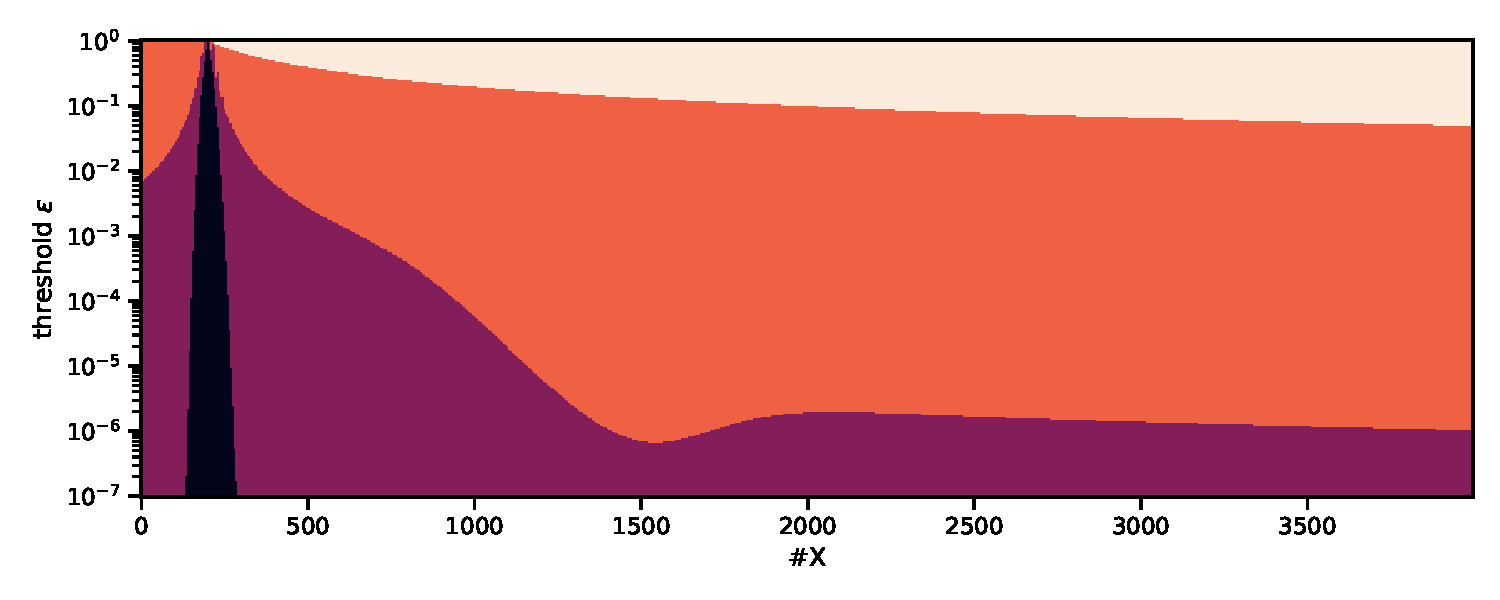
\includegraphics[width=\textwidth]{gfx/lya_sets.pdf}
	\caption[Augmented v.\ proposal Lyapunov sets]{\label{fig:lya_sets}Lyapunov sets for the birth-death process for different probability thresholds $\epsilon$ for the augmented function (orange) and the proposal (green). The ``perfect'' sets are computed using the confidence interval (red).}
\end{figure}

In \autoref{fig:improvement_lyaaug}, we compare the sets of Lyapunov subsets for varying thresholds $\epsilon$ for the proposal and the augmented function.
We observe a consistent improvement that is the strongest for smaller $\epsilon$.
The overall improvement is significantly better using the linear proposal function.
This is mainly due to the better performance of the quadratic proposal compared to the linear.
The subset sizes using the augmented function is qualitatively similar for both choices of proposal function.
\begin{figure}[htb]
	\centering
	\subfloat[Linear proposal]
	{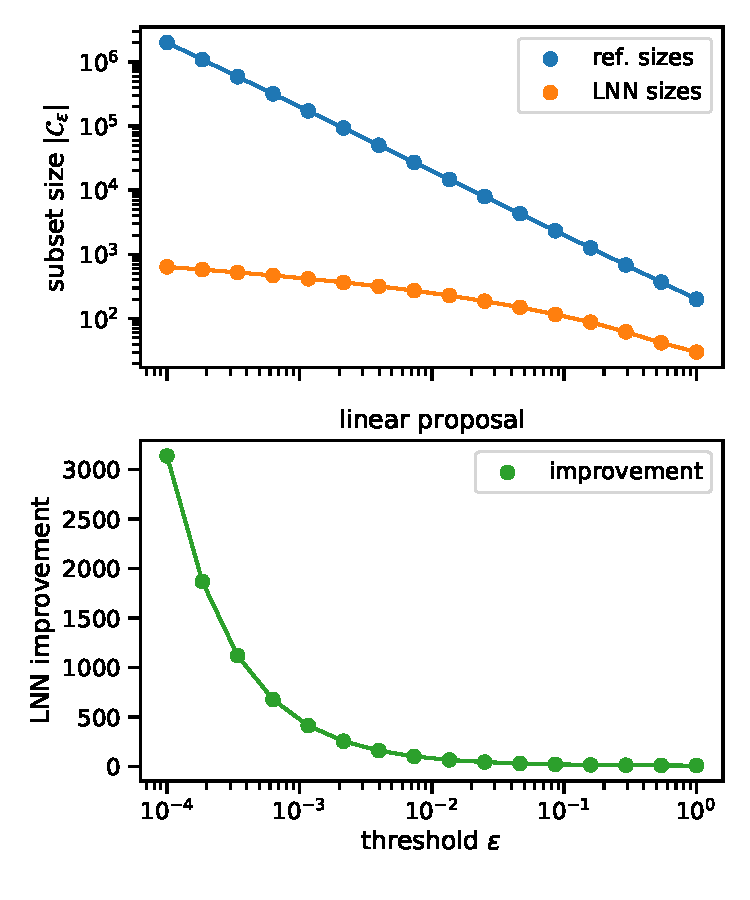
\includegraphics[width=0.48\textwidth]{gfx/lnn_improvement_linear.pdf}}
	\subfloat[Quadratic proposal]
	{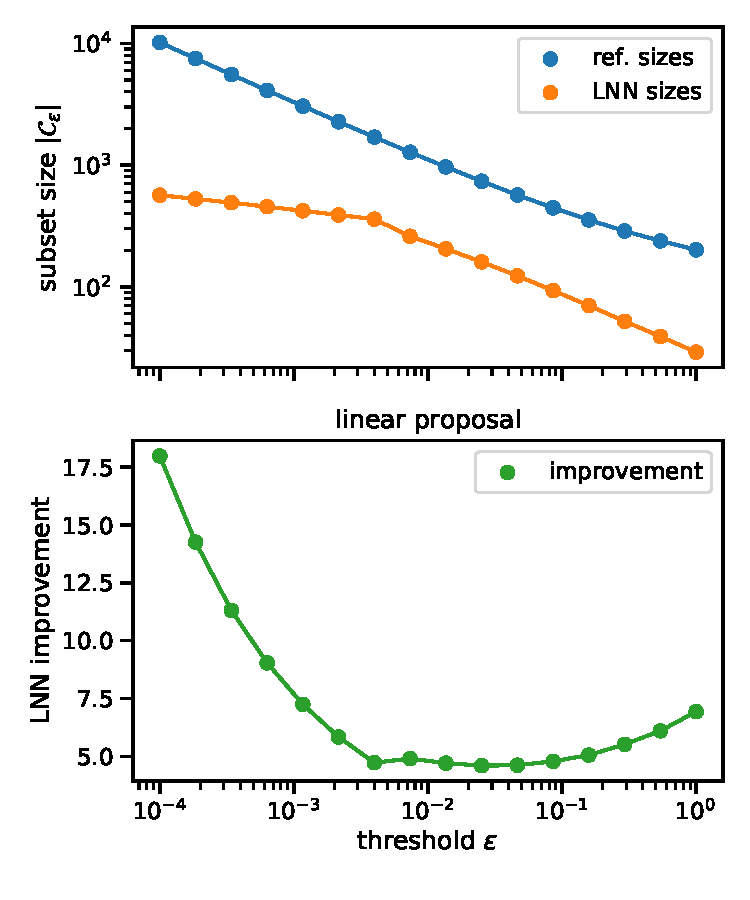
\includegraphics[width=0.48\textwidth]{gfx/lnn_improvement_quadratic.pdf}}
    \caption[Subset sizes using Lyapunov-Augmentation]{\label{fig:improvement_lyaaug}The sizes of the reference Lyapunov sets compared to the sizes of the augmented Lyapunov sets along with the improvement given by the augmentation. Results are shown for both, a linear and a quadratic proposal function.}
\end{figure}

The local augmentation of simpler proposal Lyapunov functions is promising.
To achieve more scalability and flexibility the method has some points that need refinement.
The most obvious aspect is the optimization of the local augmentation.
The evaluation of the objective necessitates the computation of the maximum drift.
In previous works this has also been directly used as an objective \parencite{milias2014optimization}.
This entails the evluation of the drift across the entire augmentation region (and some global reasoning).
Here, this issue has largely been ignored, but especially in higher dimensional models this may cause issues.
There it might be better, to estimate the maximal drift using a --~possibly random~-- grid of states instead of a dense state-space region.

Furthermore the design-space of augmentations is huge.
More conventional models may prove to be easier to handle, especially with respect to the objective computation.
Symbolic regression \parencite{pysr}, for example, may be a useful alternative to derive more explainable Lyapunov functions.

%\begin{model}[Competitive Spread]\label{model:comp_spread}
	%Two uncoupled parallel birth-death processes (cf.~\autoref{model:par_bd})\turnto{model:par_bd} supplemented with two Gray-Scott type reactions.
%%	https://groups.csail.mit.edu/mac/projects/amorphous/GrayScott/
%\begin{gather*}
    %\varnothing\xrightarrow{\rho} A\,, \quad
    %A\xrightarrow{\delta} \varnothing\,, \quad
    %\varnothing\xrightarrow{\rho} B\,, \quad
    %B\xrightarrow{\delta} \varnothing\,,\\
	%2A+B\xrightarrow{\nu_1}3A\,,\quad
	%2A+A\xrightarrow{\nu_2}3B\,.
%\end{gather*}
	%As a parameterization we choose $\rho = 5$, $\delta=0.1$, $\nu_1=\e{6}{-5}$, and $\nu_2=\e{6.2}{-5}$.
%\end{model}

